\documentclass[10pt, openright, twoside]{memoir}

\setstocksize{195mm}{130mm}
\settrimmedsize{195mm}{130mm}{*}
\setulmarginsandblock{10mm}{20mm}{*}
\setlrmarginsandblock{20mm}{10mm}{*}
\setheadfoot{10mm}{10mm}
\setheaderspaces{*}{*}{0.5}
\checkandfixthelayout{}

\usepackage{euler}

\usepackage[T1]{fontenc}
\usepackage{ETbb}
\let\oldstylenums\textosf{}

\usepackage[english]{babel}

\usepackage[none]{hyphenat}
\usepackage{lipsum}

\usepackage{float}
\usepackage{tikz}
\usetikzlibrary{arrows.meta}
\usepackage{svg}

\usepackage[stable, symbol]{footmisc}
\usepackage{amsthm}
\usepackage{amsmath}
\usepackage{physics}

\usepackage[
unicode,
pdftex,
pdfpagelabels,
bookmarks,
hyperindex,
hyperfigures,
hidelinks]{hyperref}

\renewcommand{\cftdot}{}
\addto\captionsenglish{\renewcommand{\chaptername}{bölüm}}
\addto\captionsenglish{\renewcommand{\contentsname}{içindekiler}}

\nouppercaseheads{}

\settowidth{\versewidth}{param bahçe uydular ordularla geçti}

\theoremstyle{definition}
\newtheorem*{alistirma}{alıştırma}

% \date{6 nisan 2020}

\setlength{\parindent}{5mm}
\setlength{\parskip}{2mm}

\begin{document}
\thispagestyle{empty}
\begin{flushright}
  \fontsize{0.8in}{0cm}\selectfont{}orman haydutları
\end{flushright}
\begin{flushright}
  \textit{abdullah uyu}
\end{flushright}
\vfill
\begin{figure}[H]
  \centering
  \scalebox{1.7}{
    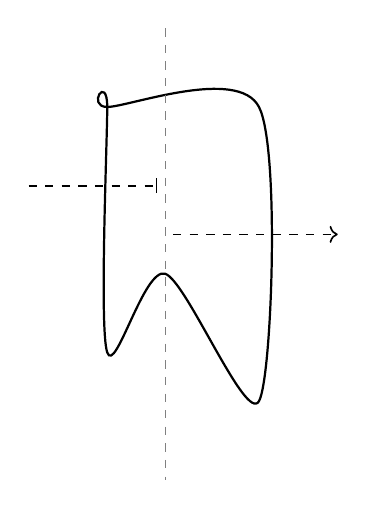
\begin{tikzpicture}
      \draw [thick] plot [smooth cycle] coordinates
      {(0, 0) (0, -3.118) (0.736, -2.118) (1.927, -3.736) (1.927, 0) (0, 0)};
      \draw [dashed, gray] (0.736, 1) -- (0.736, -4.736);
      \draw [-|, semithick, dashed] (-1, -1) -- (0.636, -1);
      \draw [->, semithick, dashed] (0.836, -1.618) -- (2.927, -1.618);
    \end{tikzpicture}}
\end{figure}
\newpage
\textbf{abdullah uyu}

17 haziran 1999'da konya'da doğdu. liseyi
konya'da okudukdan sonra üniversiteye
istanbul'a geldi. halen galatasaray
üniversitesi'nde matematik bölümü
öğrencisidir. hisarüstü'nde ikamet eder.

şiir yazmaya 2018 senesinde başladı. üç
sene kadar şiirlerini yakın çevresi dışında
paylaşmadı. 2022'de mevzular derin fanzin
ve 2023'de iğreti fanzin'de yazmaya
başlayarak şiirlerini okuyucuya açmıştır.
\newpage
\tableofcontents
\chapter{atak beş}
\topskip0pt
\vspace*{\fill}
\needspace{8\baselineskip}
\poemtitle{pipe}
\settowidth{\versewidth}{travelling along an asymptote}
\begin{verse}[\versewidth]
  think all is approximate \\
  getting more precise is \\
  travelling along an asymptote \\
  speeding up is delicate \\
  and no more useful than \\
  smoking a pipe with a mate \\
\end{verse}
\vspace*{\fill}
%
\newpage
\topskip0pt
\vspace*{\fill}
\needspace{21\baselineskip}
\poemtitle{sessiz}
\settowidth{\versewidth}{sevgim diyorum dinliyor musun}
\begin{verse}[\versewidth]
  dönüp baktım \\
  donuk baktım \\
  bir yerler var içimde \\
  sessiz ah sessiz

  ne nihavend ne hicaz \\
  ben bitkin değilim \\
  bir duygu buldum kendim \\
  sessiz ah sessiz

  çok konuştu çok düşündüm \\
  bekler yolunu üşürdüm \\
  peşinden bakakaldım o gün \\
  sessiz ah sessiz

  yoluk yitik mavi \\
  sevgim diyorum dinliyor musun \\
  bazen seni anıyorum \\
  sessiz ah sessiz
\end{verse}
\vspace*{\fill}
%
\newpage
\topskip0pt
\vspace*{\fill}
\needspace{11\baselineskip}
\poemtitle{mutuel}
\settowidth{\versewidth}{tu dois abandonner un petit peu}
\begin{verse}[\versewidth]
  tu dois abandonner un petit peu \\
  pour que tu m'aimes \\
  je vais attendre ton coup \\
  je vais t'aimer quand même

  tu dois en essayer un petit peu \\
  pour que tu m'aimes \\
  je vais attendre tes yeux \\
  je vais t'aimer quand même
\end{verse}
\vspace*{\fill}
%
\newpage
\topskip0pt
\vspace*{\fill}
\needspace{31\baselineskip}
\poemtitle{turuncu\footnote[2]{iowar'in ricası üzerine çıkarıldı.}}
\begin{verse}[\versewidth]
  \phantom{}\\
  \phantom{}\\
  \phantom{}\\
  \phantom{}\\
  \phantom{}\\
  \phantom{}\\
  \phantom{}\\
  \phantom{}\\
  \phantom{}\\
  \phantom{}\\
  \phantom{}\\
  \phantom{}\\
  \phantom{}\\
  \phantom{}\\
  \phantom{}\\
  \phantom{}\\
  \phantom{}\\
  \phantom{}\\
  \phantom{}\\
  \phantom{}\\
  \phantom{}\\
  \phantom{}\\
  \phantom{}\\
  \phantom{}\\
  \phantom{}\\
  \phantom{}\\
  \phantom{}\\
  \phantom{}\\
  \phantom{}\\
\end{verse}
\vspace*{\fill}
%
\newpage
\topskip0pt
\vspace*{\fill}
\needspace{11\baselineskip}
\poemtitle{tek harf}
\settowidth{\versewidth}{sensizlikle dost oldum}
\begin{verse}[\versewidth]
  sensizlikle dost oldum \\
  sohbetine doğum yok \\
  fikirlerim sustukça \\
  alnından tutan oldu

  sessizlikle dost oldum \\
  sohbetine doyum yok \\
  fikirlerim kustukça \\
  alnından tutar oldu
\end{verse}
\vspace*{\fill}
%
\newpage
\topskip0pt
\vspace*{\fill}
\needspace{6\baselineskip}
\poemtitle{bahar}
\settowidth{\versewidth}{bahar gelir güller açar}
\begin{verse}[\versewidth]
  bahar gelir güller açar \\
  eller güler ben gülmem \\
  her güzeli biri sever \\
  sevdim seni sümbül ben
\end{verse}
\vspace*{\fill}
%
\newpage
\topskip0pt
\vspace*{\fill}
\needspace{10\baselineskip}
\poemtitle{dertsiz}
\settowidth{\versewidth}{ne boştum ben biliyorsun}
\begin{verse}[\versewidth]
  derdin yoksa yazma dedi \\
  konuşmayı bıraktım \\
  sevme boşa koşma dedi \\
  sürekli surat astım \\
  yukarı doğru böcekler \\
  silik siyah yuvarlak \\
  ne boştum ben biliyorsun \\
  ne yüreğimi açtım
\end{verse}
\vspace*{\fill}
%
\newpage
\topskip0pt
\vspace*{\fill}
\needspace{6\baselineskip}
\poemtitle{tam}
\settowidth{\versewidth}{hiçbir şey tam değil de seni yaklaşık sanmışdım}
\begin{verse}[\versewidth]
  hiçbir şey tam değil de seni yaklaşık sanmışdım \\
  ardından esintine büyülenip sallanmışdım \\
  çok şey tam yüreğimde en eksiğim bi sen kaldım \\
  iki bakdın bi güldün aklımı elimden aldın
\end{verse}
\vspace*{\fill}
%
\newpage
\topskip0pt
\vspace*{\fill}
\needspace{6\baselineskip}
\poemtitle{factual}
\settowidth{\versewidth}{you seemed to me then really virtual}
\begin{verse}[\versewidth]
  you think i don't know the actual \\
  but you don't also talk so factual \\
  then don't judge me anymore bug \\
  you seemed to me then really virtual
\end{verse}
\vspace*{\fill}
%
\newpage
\topskip0pt
\vspace*{\fill}
\needspace{17\baselineskip}
\poemtitle{uzak}
\settowidth{\versewidth}{solgun bak ne zor görünür ya görünmez havada}
\begin{verse}[\versewidth]
  dünya güneşe ne kadar uzaksa \\
  bazı hislere o kadar uzağım \\
  eskisi gibi değil \\
  biri elli üç geçe \\
  dünya olsam da ben \\
  aşk güneş yine de \\
  çok üzücü belki \\
  ışıtıyor değil \\
  yolum var sevgiye uzun \\
  uzağım hem yol bilmem ben

  asuman sevgiye yolum bir gün gelir biter mi \\
  yoksa dün gibi izi de yarın olur yiter mi \\
  solgun bak ne zor görünür ya görünmez havada \\
  aranır bir körpe çocuk yok kaybolup gider mi
\end{verse}
\vspace*{\fill}
%
\newpage
\topskip0pt
\vspace*{\fill}
\needspace{5\baselineskip}
\poemtitle{aksiyom}
\settowidth{\versewidth}{ağlayıp sızlamaya gerek yok}
\begin{verse}[\versewidth]
  bu dünyada ne doğru var \\
  ne yanlış var ne gerçek \\
  ağlayıp sızlamaya gerek yok
\end{verse}
\vspace*{\fill}
%
\newpage
\topskip0pt
\vspace*{\fill}
\needspace{6\baselineskip}
\poemtitle{başardılar}
\settowidth{\versewidth}{bir zamanlar arkadaşdık fakat mühim değil çok}
\begin{verse}[\versewidth]
  sevdiğim bazı şeyler var nedir hiç önemi yok \\
  insanlar onlardan nefret etmeyi başardılar \\
  bir zamanlar arkadaşdık fakat mühim değil çok \\
  inatla benden de nefret etmeyi başardılar
\end{verse}
\vspace*{\fill}
%
\newpage
\topskip0pt
\vspace*{\fill}
\needspace{6\baselineskip}
\poemtitle{aşamamışım}
\settowidth{\versewidth}{bilmem niye durduk yere benim üzülmelerim}
\begin{verse}[\versewidth]
  diyebilirsin ki dünle benim problemlerim \\
  aşamamışım onları ben atlatamamışım \\
  bilmem niye durduk yere benim üzülmelerim \\
  eski kaset çalarlara dönüp bakamayışım
\end{verse}
\vspace*{\fill}
%
\newpage
\topskip0pt
\vspace*{\fill}
\needspace{6\baselineskip}
\poemtitle{a\~nız}
\settowidth{\versewidth}{derin derin göğe bak ve}
\begin{verse}[\versewidth]
  ağzı\~nda a\~nız dolu  \\
  bir tarlada yalınayak  \\
  derin derin göğe bak ve \\
  de ki dünya ne garip.
\end{verse}
\vspace*{\fill}
%
\newpage
\topskip0pt
\vspace*{\fill}
\needspace{6\baselineskip}
\poemtitle{saçlarına çal beni}
\settowidth{\versewidth}{dört bi yana saçık olsam}
\begin{verse}[\versewidth]
  havadaki ışık olsam \\
  dört bi yana saçık olsam \\
  saçlarına çalık olsam \\
  yine de doyamam sana
\end{verse}
\vspace*{\fill}
%
\newpage
\topskip0pt
\vspace*{\fill}
\needspace{6\baselineskip}
\poemtitle{fikirler de pernelir}
\settowidth{\versewidth}{şu lanet yurt odasında}
\begin{verse}[\versewidth]
  göğün yüzü turuncuyor \\
  fikirlerim perleniyor \\
  tüm bedenim çürüyor \\
  şu lanet yurt odasında
\end{verse}
\vspace*{\fill}
%
\newpage
\topskip0pt
\vspace*{\fill}
\needspace{14\baselineskip}
\poemtitle{portakal esen rüzgar}
\settowidth{\versewidth}{bırakıp beynimi fikir sellerine}
\begin{verse}[\versewidth]
  portakal esen rüzgarı \\
  gülüşüne düğümledin \\
  çözmezsen zamanı \\
  bakar dururum ellerine \\
  dönüp arkanı yürüdün \\
  bırakıp beynimi fikir sellerine \\
  yavaşça oku söylediklerimi \\
  bilirsin çok zekiyim ama \\
  sana karşı mantıklı olamıyorum \\
  duygularım konuşuyor gözlerine \\
  düşünemiyorum bakarken \\
  güzel yüzüyü\~n ferine
\end{verse}
\vspace*{\fill}
%
\newpage
\topskip0pt
\vspace*{\fill}
\needspace{13\baselineskip}
\poemtitle{hududunda dünlerin}
\settowidth{\versewidth}{artık bir güz rüzgarı}
\begin{verse}[\versewidth]
  artık bir güz rüzgarı \\
  esiyorsun sen sarı \\
  sevda ile sonuncu \\
  kahverengi turuncu

  hüzünle sensizliğin \\
  fikrine bakıyorum \\
  sukünetle oturup \\
  hududunda dünlerin \\
  seni hatırlıyorum \\
  seyri\~ne dalıyorum
\end{verse}
\vspace*{\fill}
%
\newpage
\topskip0pt
\vspace*{\fill}
\needspace{16\baselineskip}
\poemtitle{is}
\settowidth{\versewidth}{kalbimde tozuyan küllerde buldum}
\begin{verse}[\versewidth]
  havadaki gızıl iste aradım \\
  kalbimde tozuyan küllerde buldum \\
  sabanı\~n serin yelinde aradım \\
  başımdaki sevda yelinde buldum

  kağıttaki mürekkepte aradım \\
  damarlarımda akan kanda buldum \\
  aşkla öten bülbüllerde aradım \\
  beynimdeki sesimde buldum seni

  nedeni bilinmez mahzun yüzüne \\
  çaresizmişsin garip hallerine \\
  dönüp kendime yorgun bedenime \\
  bakıyorum yazık ettim diyorum.
\end{verse}
\vspace*{\fill}
%
\newpage
\topskip0pt
\vspace*{\fill}
\needspace{16\baselineskip}
\poemtitle{perdeler}
\settowidth{\versewidth}{gönlümde sen parlarsın}
\begin{verse}[\versewidth]
  turuncayan gökleri \\
  izledinse anlarsın \\
  sevgin öyle kalbimde \\
  yıldızları perdeler

  erinceyen yıllardır \\
  gönlümde sen parlarsın \\
  yüzün öyle kalbimde \\
  kızgın çöller perdeler

  evrilen yazıların \\
  harflerini çatarsın \\
  sesin öyle kalbimde \\
  küt düğümler perdeler
\end{verse}
\vspace*{\fill}
%
\newpage
\topskip0pt
\vspace*{\fill}
\needspace{27\baselineskip}
\poemtitle{asumanla muhabbet}
\settowidth{\versewidth}{o sevdanı\~n yelidir.}
\begin{verse}[\versewidth]
  bana bak göğün yüzü \\
  sen turuncu olunca \\
  varsa eğer başımda \\
  biraz akıl gidiyor

  zaten sana bakarım \\
  turuncayıp akarım \\
  tek gördüğüm başında \\
  o sevdanı\~n yelidir.

  bir mazlım çocuğudum \\
  evtikler oturudum \\
  onu da bilmezidim \\
  gene de gideridi.

  sevda zamanla gelmez \\
  leyla amanla sevmez \\
  o yüzden gideridi \\
  değerli güzel aklı\~n

  seni a\~nlamak zormuş \\
  turuncayan gö\~nülde \\
  parıldayan o kormuş \\
  anladım benim gibi \\
  seni de biri yormuş
\end{verse}
\vspace*{\fill}
%
\newpage
\topskip0pt
\vspace*{\fill}
\needspace{12\baselineskip}
\poemtitle{taşlarlar}
\settowidth{\versewidth}{bugün akıl var sanrı yok.}
\begin{verse}[\versewidth]
  bugün akıl var sanrı yok. \\
  güneş var kölge var. \\
  yiğit var er var. \\
  sevgi var yar yok. \\
  o yüzden  \\
  gelme tekrar aklıma \\
  geçme gönül semtimden \\
  görürse fikirlerim \\
  taşlarlar yüreğini \\
  razı olmam yanmana
\end{verse}
\vspace*{\fill}
%
\newpage
\topskip0pt
\vspace*{\fill}
\needspace{16\baselineskip}
\poemtitle{beynemaz}
\settowidth{\versewidth}{$\mathcal{L}(U, V)$ kategori}
\begin{verse}[\versewidth]
  bildim $f$ lipschitzienne \\
  $\mathcal{L}(U, V)$ kategori \\
  geçirdim tüm vakiti \\
  dönüştüm beynemaza

  kitabına yüz sürdüm \\
  türevli denklem bildim \\
  ispat arayıp gezdim \\
  dönüştüm beynemaza

  karanlık aydınlığa \\
  soluk güzler bahara \\
  dönsün diye dönüştüm \\
  dönüştüm beynemaza
\end{verse}
\vspace*{\fill}
%
\newpage
\topskip0pt
\vspace*{\fill}
\needspace{11\baselineskip}
\poemtitle{yüreğiyi\~n tahtını\~n kolçağı}
\settowidth{\versewidth}{düşsem bir gün kalbi\~ne}
\begin{verse}[\versewidth]
  parçalasam tersine \\
  dönen tüm kasnakları \\
  düşsem bir gün kalbi\~ne \\
  çıksam basamakları

  yükselip yüreğiyi\~n \\
  tahtına nazar etsem \\
  yürüsem kolçağına \\
  bakarak sersem sersem
\end{verse}
\vspace*{\fill}
%
\newpage
\topskip0pt
\vspace*{\fill}
\needspace{6\baselineskip}
\poemtitle{yetki}
\settowidth{\versewidth}{bir yetkim yok anladım}
\begin{verse}[\versewidth]
  bir yetkim yok anladım \\
  hayatım üzerine \\
  ömrümce bakacağım \\
  o güzel gözlerine
\end{verse}
\vspace*{\fill}
%
\newpage
\topskip0pt
\vspace*{\fill}
\needspace{6\baselineskip}
\poemtitle{küreler}
\settowidth{\versewidth}{zannediyorum çok küre kıra kıra bura geldim}
\begin{verse}[\versewidth]
  zannediyorum çok küre kıra kıra bura geldim \\
  sorma bana doğruyu yanlışı aklı erdemi \\
  fakat bu sonuncunun kör etti dağılan bendi \\
  bilmem dışarda mıyım söyle yoksa içerde mi
\end{verse}
\vspace*{\fill}
%
\newpage
\topskip0pt
\vspace*{\fill}
\needspace{6\baselineskip}
\poemtitle{küllerini gönlüne sar}
\settowidth{\versewidth}{bulamam senin gibi hem güzel hem sözleri bal}
\begin{verse}[\versewidth]
  yakarım al sesimi küllerini gönlüne sar \\
  beyaz mavi yeşil mor boyanıp da gönlüme dal \\
  oyalanma uzakta ah gel beraber gezelim \\
  bulamam senin gibi hem güzel hem sözleri bal
\end{verse}
\vspace*{\fill}
%
\newpage
\topskip0pt
\vspace*{\fill}
\needspace{13\baselineskip}
\poemtitle{türev}
\begin{alistirma}
  \(\mathcal{T}\), kanonik üzüntüler uzayından bir travma olmak üzere,
  \[
    \dv{\mathcal{T}}
    \left(
      \begin{tabular}{l}
        göğsümün sol tarafı \\
        yanıyor arkadaşım \\
        ığranmaz yapraklarla \\
        incitmez kollarımı \\
        boş hayal sessiz ölüm
      \end{tabular}
    \right)
    =
    \begin{tabular}{l}
      kıstırıp solda rafı \\
      kanıyor aşka başım \\
      fırlatsak çardakları \\
      siğdirmez bollarını \\
      koş sağa eşsiz ömür
    \end{tabular}
  \]
  eşitliği veriliyor. $\mathcal{T}$'yi kendi travmalarınız cinsinden ifade
  ediniz.
\end{alistirma}
\vspace*{\fill}
%
\newpage
\topskip0pt
\vspace*{\fill}
\needspace{6\baselineskip}
\poemtitle{yakışık}
\settowidth{\versewidth}{isteğim bana kendinden başka bir arkadaş ver}
\begin{verse}[\versewidth]
  ben böyle tek başıma yürümek istemiyorum \\
  isteğim bana kendinden başka bir arkadaş ver \\
  ne gülmek belli ne ağlamak huzur istiyorum \\
  isteğim bana kendinden başka bir arkadaş ver
\end{verse}
\vspace*{\fill}
%
\newpage
\topskip0pt
\vspace*{\fill}
\needspace{10\baselineskip}
\poemtitle{istemediklerim}
\settowidth{\versewidth}{her gün senden daha fazla}
\begin{verse}[\versewidth]
  severken insanlığıma \\
  imtihan istemedim \\
  dertsiz tasasız başıma \\
  sıkıntı istemedim \\
  her gün senden daha fazla \\
  kaçmayı istemedim \\
  çık işte gönül bahçemden \\
  çık kurtulayım senden
\end{verse}
\vspace*{\fill}
%
\newpage
\topskip0pt
\vspace*{\fill}
\needspace{6\baselineskip}
\poemtitle{terzi}
\settowidth{\versewidth}{sessiz sakin bir yerde}
\begin{verse}[\versewidth]
  iplik iğne ve kumaş \\
  oturup keseceğim \\
  sessiz sakin bir yerde \\
  defterler dikeceğim
\end{verse}
\vspace*{\fill}
%
\newpage
\topskip0pt
\vspace*{\fill}
\needspace{6\baselineskip}
\poemtitle{beşik}
\settowidth{\versewidth}{sonra sarardın sen de üzüldün baktık ardından}
\begin{verse}[\versewidth]
  pek güzel bir gün idin rüzgarınla güneşinle \\
  güldük koştuk eğlendik kollarında beşiğinde \\
  sonra sarardın sen de üzüldün baktık ardından \\
  gitme bizi bırakma buruk kalpler eşiğinde
\end{verse}
\vspace*{\fill}
%
\newpage
\topskip0pt
\vspace*{\fill}
\needspace{14\baselineskip}
\poemtitle{arkadaş}
\settowidth{\versewidth}{biraz kalem biraz defter konuşsun}
\begin{verse}[\versewidth]
  looking for a friend \\
  speaks geek and some poem \\
  wandering around \\
  proximity of you close in \\
  with the hope of \\
  a coincidence genuine

  bir arkadaş arıyorum \\
  biraz kalem biraz defter konuşsun \\
  çevrende dolaşıyorum \\
  ümidiyle bir rastlantı \\
  bi an gelsin sözlerimiz buluşsun
\end{verse}
\vspace*{\fill}
%
\newpage
\topskip0pt
\vspace*{\fill}
\needspace{11\baselineskip}
\poemtitle{leylaya}
\settowidth{\versewidth}{mutluydum bıktım bak dert sahibi artık bu gemi}
\begin{verse}[\versewidth]
  boğulmak bana yakışmıyor sil gözyaşlarımı \\
  otur karşımda ya da gel ağlayalım sarılıp \\
  savrulacak yanıma boş bir deryaya karılıp \\
  ne yakınım ne sevgilim ne de dostum var benim

  aradım yıllardır fakat bulamadım gülşeni \\
  mutluydum bıktım bak dert sahibi artık bu gemi \\
  bil ki çok yorgunum bekleme bu halde gülmemi \\
  ne huzurum ne sevincim ne de aklım var benim \\
\end{verse}
\vspace*{\fill}
%
\newpage
\topskip0pt
\vspace*{\fill}
\needspace{6\baselineskip}
\poemtitle{şaheser}
\settowidth{\versewidth}{fersiz nemli gözlerim sor kimin eseridir}
\begin{verse}[\versewidth]
  bitirdim mürekkebi kanım katsam yeridir \\
  fersiz nemli gözlerim sor kimin eseridir \\
  senin aşkın ölümün bir diğer bedenidir \\
  fersiz nemli gözlerim sor kimin eseridir
\end{verse}
\vspace*{\fill}
%
\newpage
\topskip0pt
\vspace*{\fill}
\needspace{6\baselineskip}
\poemtitle{kar yağar}
\settowidth{\versewidth}{kar yağar yağmur yağar}
\begin{verse}[\versewidth]
  sen üzülme güzelim \\
  ikimiz üzülürsek \\
  kar yağar yağmur yağar \\
  taşar gönlüm sel olur
\end{verse}
\vspace*{\fill}
%
\newpage
\topskip0pt
\vspace*{\fill}
\needspace{11\baselineskip}
\poemtitle{gazel}
\settowidth{\versewidth}{siz de sürüklenmeyin}
\begin{verse}[\versewidth]
  durun orda gazeller \\
  siz de sürüklenmeyin \\
  benim sevda yolunda \\
  sürüklendiğim gibi

  bir yalanın önünden \\
  bir güzelin peşinden \\
  yolun sonun bilmeden \\
  koşup gittiğim gibi
\end{verse}
\vspace*{\fill}
%
\newpage
\topskip0pt
\vspace*{\fill}
\needspace{6\baselineskip}
\poemtitle{gaye}
\settowidth{\versewidth}{gel peşimden bilinmeze gidelim}
\begin{verse}[\versewidth]
  gel peşimden bilinmeze gidelim \\
  sevda içip kayıp çölde gezelim \\
  sarhoşluğun belirsiz gayesiyle \\
  arayalım sevgiyi raks edelim
\end{verse}
\vspace*{\fill}
%
\newpage
\topskip0pt
\vspace*{\fill}
\needspace{17\baselineskip}
\poemtitle{tanrı seni korusun}
\settowidth{\versewidth}{hatta sen tüm evrenin}
\begin{verse}[\versewidth]
  önce kendi çevrenin \\
  sonra bütün beldenin \\
  hatta sen tüm evrenin \\
  bulunmaz çiçeğisin

  rüzgar sağa sapmalı \\
  ışık senden kaçmalı \\
  nerede saklamalı \\
  sararır üzülürsün

  kolayca bilinmekten \\
  hisleri sezilmekten \\
  herkese görünmekten \\
  tanrı seni korusun \\
  tanrı seni korusun
\end{verse}
\vspace*{\fill}
%
\newpage
\topskip0pt
\vspace*{\fill}
\needspace{6\baselineskip}
\poemtitle{hicran}
\settowidth{\versewidth}{damla damla hicransın gözümde aylardır leyla}
\begin{verse}[\versewidth]
  damla damla hicransın gözümde aylardır leyla \\
  ağlayıp dökmekle bitsen ah bitiremiyorum \\
  günlerim aşkını içmekle geçse de belirsiz \\
  ne tam sarhoş geziyorum ne tam ayığım leyla
\end{verse}
\vspace*{\fill}
%
\newpage
\topskip0pt
\vspace*{\fill}
\needspace{7\baselineskip}
\poemtitle{aklıma geldin}
\settowidth{\versewidth}{karşıda çamlar soruyor ne gözlerinin rengi}
\begin{verse}[\versewidth]
  gün battı gökyüzü mavi yine aklıma geldin \\
  bulanık sadece ay var yüreğimi açacak \\
  karşıda çamlar soruyor ne gözlerinin rengi \\
  gözlerinin rengidir ne nazarımdan kaçacak \\
  ne cesaretim var sana ilgimi anlatacak
\end{verse}
\vspace*{\fill}
%
\newpage
\topskip0pt
\vspace*{\fill}
\needspace{6\baselineskip}
\poemtitle{mütekerrir}
\settowidth{\versewidth}{ben istiyorum bitsin bu mütekerrir hicranım}
\begin{verse}[\versewidth]
  ben istiyorum bitsin bu mütekerrir hicranım \\
  yoktur bulamıyorum derman biçare derdine \\
  hem dalıyorum bir saba şarkı ile bitabım \\
  yokluğunun bulutları bak yeniden geldiler
\end{verse}
\vspace*{\fill}
%
\newpage
\topskip0pt
\vspace*{\fill}
\needspace{10\baselineskip}
\poemtitle{param bahçe}
\settowidth{\versewidth}{senden bir ses bekledim gel konuşalım diyecek}
\begin{verse}[\versewidth]
  param bahçe uydular ordularla geçti küller \\
  senden bir ses bekledim gel konuşalım diyecek \\
  ne gülebiliyordum ne iştah vardı yiyecek \\
  param bahçe uydular ordularla geçti küller \\
  geçgi dünler \\
  dengi güçler \\
  geçdi günler \\
  paramparça uykular korkularla geçti günler
\end{verse}
\vspace*{\fill}
%
\newpage
\topskip0pt
\vspace*{\fill}
\needspace{6\baselineskip}
\poemtitle{kalem kağıt mürekkep}
\settowidth{\versewidth}{kalem kağıt mürekkep}
\begin{verse}[\versewidth]
  kalem kağıt mürekkep \\
  şiir yazar dururdum \\
  peşinde dolaşmaktan \\
  güzelim çok yoruldum
\end{verse}
\vspace*{\fill}
%
\newpage
\topskip0pt
\vspace*{\fill}
\needspace{16\baselineskip}
\poemtitle{bulanlar}
\settowidth{\versewidth}{bir gün sevmek isteyip}
\begin{verse}[\versewidth]
  bir gün sevmek isteyip \\
  yollarımı beklersen \\
  yerde sarı gazele \\
  sor acaba nerdeyim

  sevda içip aşkınla \\
  kayıp çölde gezersen \\
  yerde toza toprağa \\
  sor acaba nerdeyim

  sıkılıp bunalırsın \\
  aramakla bulunmam \\
  bulanları keşfedip \\
  sor acaba nerdeyim
\end{verse}
\vspace*{\fill}
%
\newpage
\topskip0pt
\vspace*{\fill}
\needspace{11\baselineskip}
\poemtitle{herkes gibi}
\settowidth{\versewidth}{ben de herkes gibi aşık oldum sana}
\begin{verse}[\versewidth]
  ben de herkes gibi aşık oldum sana \\
  bambaşka başladı aynı bitti işte \\
  bakıp gökyüzünü yüze anımsamam \\
  eritti tüketti yaktı beni işte

  sözlerinden geçip kaçamıyorum \\
  gidilecek yol var alamıyorum \\
  aşkını kalbimden söküp atsam da \\
  söndürüp külünü saçamıyorum
\end{verse}
\vspace*{\fill}
%
\newpage
\topskip0pt
\vspace*{\fill}
\needspace{6\baselineskip}
\poemtitle{elde varken}
\settowidth{\versewidth}{elde varken tüm aklımı tükettim}
\begin{verse}[\versewidth]
  elde varken tüm aklımı tükettim \\
  yokluğunda sinirlendim pişmanım \\
  iyiliği sabahları aradım \\
  akşam olup üzüntüyle yanarım
\end{verse}
\vspace*{\fill}
%
\newpage
\chapter{bahariye ön dört taksim üç}
\topskip0pt
\vspace*{\fill}
\needspace{8\baselineskip}
\poemtitle{sen de bi küreydin}
\settowidth{\versewidth}{bir garipken yankılanan}
\begin{verse}[\versewidth]
  bir garipken yankılanan \\
  yüreğinin çeperinde \\
  kırıp sevda küresini \\
  çıkıp izlerime baktım \\
  paramparça o evreni \\
  unutmak nehrine attım
\end{verse}
\vspace*{\fill}
%
\newpage
\topskip0pt
\vspace*{\fill}
\needspace{6\baselineskip}
\poemtitle{tekrar tekrar}
\settowidth{\versewidth}{o kadar çok şey var ki sana dair bilmediğim}
\begin{verse}[\versewidth]
  her aklıma geldiğinde bir şiir yazıyorum \\
  yokluğunu kalbime tekrar tekrar kazıyorum \\
  o kadar çok şey var ki sana dair bilmediğim \\
  bazı zaman gizeminden kaçarak yaşıyorum
\end{verse}
\vspace*{\fill}
%
\newpage
\topskip0pt
\vspace*{\fill}
\needspace{11\baselineskip}
\poemtitle{üşengeç}
\settowidth{\versewidth}{tüm çer çöp çarpar sana}
\begin{verse}[\versewidth]
  kıpırdamayan taşsın \\
  sen efkar nehrimde \\
  tüm çer çöp çarpar sana \\
  dersin üstümden aşsın

  üzülüp yüreğime \\
  yerinden ayaklansan \\
  bu sefer sel götürür \\
  kaldırmaz gönlüm aklım
\end{verse}
\vspace*{\fill}
%
\newpage
\topskip0pt
\vspace*{\fill}
\needspace{6\baselineskip}
\poemtitle{rayhânasa}
\settowidth{\versewidth}{akar kalbim seyreline}
\begin{verse}[\versewidth]
  günben güne âhefbine \\
  akar kalbim seyreline \\
  bilmun olsa rayhânasa \\
  bakar berum feyrenine
\end{verse}
\vspace*{\fill}
%
\newpage
\topskip0pt
\vspace*{\fill}
\needspace{22\baselineskip}
\poemtitle{kalanlar}
\settowidth{\versewidth}{hem anlatsaydın ne vardı}
\begin{verse}[\versewidth]
  şimdileri neş'enin \\
  yerini sessizlik aldı \\
  pür sevgimden geriye \\
  bir garip üzüntün kaldı

  halini gelip bana \\
  hem anlatsaydın ne vardı \\
  geçen baygın günlerim \\
  hep bana hatıra kaldı \\
  pür sevgimden geriye \\
  bir garip üzüntün kaldı

  yüzünü görmemekle \\
  unutulup sen gitmezsin \\
  sen gülmezsen hem eğer \\
  bu üzüntüm nasıl geçsin \\
  söyle bana çekinme \\
  ah söyle sen kaç dizesin \\
  saklanıp efkarımla \\
  yazıp bitiremiyorum
\end{verse}
\vspace*{\fill}
%
\newpage
\topskip0pt
\vspace*{\fill}
\needspace{16\baselineskip}
\poemtitle{sevgi}
\settowidth{\versewidth}{sar belinden bir gülşenin yorgun kolların açıp}
\begin{verse}[\versewidth]
  sevgi darmadağın edip erittikden sonra ah \\
  usanmayıp gözlerinden hoş gülmeni bekliyor \\
  yavaşca arkandan gelip bir güzel bul ona bak \\
  erinceyen şu kalbini durma aşık et diyor

  bırak şu serseriliği sevda yoluna bakıp \\
  bul bi tane aşk beşiği derin gülüşler aşıp \\
  sar belinden bir gülşenin yorgun kolların açıp \\
  yorgun kollar iyileşir durma aşık ol diyor

  güzel yoksa etrafında inan ki boş bu cihan \\
  tüm dünyanı süsler ondan gelen yitik bir nigah \\
  bir sağa git bir sola dön dolaş sen onu an \\
  var yanına iltifat et durma aşık ol diyor
\end{verse}
\vspace*{\fill}
%
\newpage
\topskip0pt
\vspace*{\fill}
\needspace{6\baselineskip}
\poemtitle{bold}
\settowidth{\versewidth}{lazy looking luxury lacks}
\begin{verse}[\versewidth]
  bipolar bitch being bold \\
  dull disaster doing deck \\
  lazy looking luxury lacks \\
  righteous roundly relax
\end{verse}
\vspace*{\fill}
%
\newpage
\topskip0pt
\vspace*{\fill}
\needspace{6\baselineskip}
\poemtitle{o zamanlar}
\settowidth{\versewidth}{rüzgar arkamda mehtap sarıydı}
\begin{verse}[\versewidth]
  o zamanlar bağ üzüm bağıydı \\
  düşer önüne aşkın yürürdüm \\
  rüzgar arkamda mehtap sarıydı \\
  bekler yolunu kalbim sürürdüm
\end{verse}
\vspace*{\fill}
%
\newpage
\topskip0pt
\vspace*{\fill}
\needspace{10\baselineskip}
\poemtitle{belli belirsiz}
\settowidth{\versewidth}{hem önemli hem önemsiz}
\begin{verse}[\versewidth]
  bazen seni düşünürken \\
  gökte belli belirsiz \\
  uzak sarı turuncayan \\
  dumanlar görüyorum \\
  gölgesinde gördüğümün \\
  bir sokakta yürürken \\
  hem önemli hem önemsiz \\
  her şeyden geçiyorum
\end{verse}
\vspace*{\fill}
%
\newpage
\topskip0pt
\vspace*{\fill}
\needspace{6\baselineskip}
\poemtitle{arkadaşım ve arkadaşının}
\settowidth{\versewidth}{sana izin veriyorum}
\begin{verse}[\versewidth]
  sakın bağırma bana \\
  bağırabilirsin ama \\
  sana izin veriyorum \\
  ama sadece sana
\end{verse}
\vspace*{\fill}
%
\newpage
\topskip0pt
\vspace*{\fill}
\needspace{6\baselineskip}
\poemtitle{iki iki}
\settowidth{\versewidth}{bana bir yar galiba şu kıpkızıl güneş kaldı}
\begin{verse}[\versewidth]
  bu ikindi her şeyi iki iki görüyorum \\
  bana bir yar galiba şu kıpkızıl güneş kaldı \\
  temelli iyileşmek ta başından görmüyordum \\
  fakat hiç bırakmadın aklımı çok kötü aldın
\end{verse}
\vspace*{\fill}
%
\newpage
\topskip0pt
\vspace*{\fill}
\needspace{14\baselineskip}
\poemtitle{solgun dolaşıyorum}
\settowidth{\versewidth}{görüp kalbi binbir göçük}
\begin{verse}[\versewidth]
  bazen gözlerinden kaçıp \\
  saklanmak istiyorum \\
  bazen sözlerini alıp \\
  göğsüme katıyorum \\
  aklımı yerlere saçıp \\
  solgun dolaşıyorum \\
  usulü ile unutup \\
  senden geçemiyorum \\
  aklımı yerlere saçıp \\
  bazen gözlerinden kaçıp \\
  görüp kalbi binbir göçük \\
  senden geçemiyorum
\end{verse}
\vspace*{\fill}
%
\newpage
\topskip0pt
\vspace*{\fill}
\needspace{6\baselineskip}
\poemtitle{disjonction cas}
\settowidth{\versewidth}{bu halimi baştan bilsem yine sevmek isterdim}
\begin{verse}[\versewidth]
  tümümden geçip senin kendimi sevgine serdim \\
  bu halimi baştan bilsem yine sevmek isterdim \\
  göz görmez kulak duymaz ah düşünmez biserdim \\
  bu halimi baştan bilsem yine sevmek isterdim \\
\end{verse}
\vspace*{\fill}
%
\newpage
\topskip0pt
\vspace*{\fill}
\needspace{6\baselineskip}
\poemtitle{aşka başım}
\settowidth{\versewidth}{sen en sevdiğim şiir arkadaşım}
\begin{verse}[\versewidth]
  sen en sevdiğim şiir arkadaşım \\
  daha hiç cevabından gocunmadım \\
  ne zaman kanasa hem aşka başım \\
  yanımda yanımda sen yanımdasın \\
\end{verse}
\vspace*{\fill}
%
\newpage
\topskip0pt
\vspace*{\fill}
\needspace{6\baselineskip}
\poemtitle{aşk küresi parlayıncazık}
\settowidth{\versewidth}{düşerim sevgiyle bir kez baksan heyecanından}
\begin{verse}[\versewidth]
  düşerim sevgiyle bir kez baksan heyecanından \\
  evren-i hayalime ben bakarak kaybolurum \\
  göğsümdeki aşk küresi parlar birden harından \\
  kaynar sinemde kanım da hüsnünde yok olurum \\
\end{verse}
\vspace*{\fill}
%
\newpage
\topskip0pt
\vspace*{\fill}
\needspace{11\baselineskip}
\poemtitle{intentionally left blank}
\settowidth{\versewidth}{i behold their books for ages}
\begin{verse}[\versewidth]
  i presume i am \\
  one of those pages \\
  intentionally left blank \\
  i matter as a whole \\
  i space-fill place-hold \\
  but nothing more \\
  i behold their books for ages \\
  so it is that reader \\
  rendering me sore \\
\end{verse}
\vspace*{\fill}
%
\newpage
\topskip0pt
\vspace*{\fill}
\needspace{8\baselineskip}
\poemtitle{sakınılacaklar}
\settowidth{\versewidth}{bir coşar bir dalgın kor onunki benzemez aşka}
\begin{verse}[\versewidth]
  durmaz işte orda da gözler yine yerde başka \\
  bir coşar bir dalgın kor onunki benzemez aşka \\
  bir girift muhabbette sakın ondan sözlerini \\
  bir kez sarhoş ayrılma geçirip günleri baygın \\
  bilinmez bir haline bağlanıp da gözlerini \\
  oyma kalbinin sonra dolu da onmaz ah boş da \\
\end{verse}
\vspace*{\fill}
%
\newpage
\topskip0pt
\vspace*{\fill}
\needspace{10\baselineskip}
\poemtitle{gizemin --- öztanıma son çağrı}
\settowidth{\versewidth}{\textit{sevgim} ve bilmediğim duygularından başka}
\begin{verse}[\versewidth]
  \textit{sevgim} ve bilmediğim duygularından başka \\
  bir kere istemedim tanımak \\
  ne ben tanıyorum seni şimdi \\
  ne de sen ben kimim biliyorsun \\
  hayal dünyamın en garip yerinde varlığın \\
  ağırlığı aşkının çoktürdüyse de bir zaman \\
  ne \textit{sevgim} diyorum seni \\
  ne de o gizemini siliyorsun \\
\end{verse}
\vspace*{\fill}
%
\newpage
\topskip0pt
\vspace*{\fill}
\needspace{6\baselineskip}
\poemtitle{hamdım pişdim hamdım\footnote[2]{anagramatikdir.}}
\settowidth{\versewidth}{afraid reine war wang}
\begin{verse}[\versewidth]
  afraid reine war wang \\
  defrag win aware rain \\
  frage drain ware wain \\
  raw refined raw again \\
\end{verse}
\vspace*{\fill}
%
\newpage
\topskip0pt
\vspace*{\fill}
\needspace{20\baselineskip}
\poemtitle{kabımız --- gece vakti ``{\ttfamily{}sort -R}'' eylençesi}
\settowidth{\versewidth}{ancak üzüntüden kaçmağa gücümüz yeter}
\begin{verse}[\versewidth]
  dolaşırız avareyiz \\
  sanki daha büyük bi kap bulduk \\
  o da biter paramparçayız işte \\
  oturup düşünmeğe vaktimiz dar \\
  ancak üzüntüden kaçmağa gücümüz yeter \\
  şimdi bulsak da eksiğiz \\
  bi orada bi burda \\
  kabımıza sığamadık da \\
  saçıldık dağıldık işte \\
  ancak üzüntüden kaçmağa gücümüz yeter \\
  dolaşırız avareyiz \\
  saçıldık dağıldık işte \\
  kabımıza sığamadık da \\
  oturup düşünmeğe vaktimiz dar \\
  bi orada bi burda \\
  o da biter paramparçayız işte \\
  sanki daha büyük bi kap bulduk \\
  şimdi bulsak da eksiğiz \\
\end{verse}
\vspace*{\fill}
%
\newpage
\topskip0pt
\vspace*{\fill}
\needspace{6\baselineskip}
\poemtitle{yeteri}
\settowidth{\versewidth}{başından sonuna kadar durmasam hiç ağlasam}
\begin{verse}[\versewidth]
  tüm nihavend şarkıları birbirine ulasam \\
  başından sonuna kadar durmasam hiç ağlasam \\
  gündüzleri gece etsem akşamları bağlasam \\
  gene yine sevgin etmez tarif-i aşka yetmez \\
\end{verse}
\vspace*{\fill}
%
\newpage
\topskip0pt
\vspace*{\fill}
\needspace{15\baselineskip}
\poemtitle{dahada değiliz}
\settowidth{\versewidth}{yorgunluk sağı içimizden}
\begin{verse}[\versewidth]
  boş bi otobüs durağı \\
  ıslak bi defter \\
  yağmurlar ancak sağanak \\
  sonbahar geliyor \\
  dahası ardı kış \\
  onu da biliyoruz \\
  yorgunluk sağı içimizden \\
  olmamak geliyor \\
  daha da ardışık \\
  dahada değiliz \\
  daha da değiliz \\
  fenikmek solu \\
  solduk \\
\end{verse}
\vspace*{\fill}
%
\newpage
\topskip0pt
\vspace*{\fill}
\needspace{6\baselineskip}
\poemtitle{kim yanar kim eksilir}
\settowidth{\versewidth}{işte ben o havaydım çevrendeydim durdum her an}
\begin{verse}[\versewidth]
  senin ateş olduğun inanıyorum hakikat \\
  hava elzem yanmakda sen de biliyorsun fakat \\
  işte ben o havaydım çevrendeydim durdum her an \\
  tükendim sen yan diye eksildim öldüm her an \\
\end{verse}
\vspace*{\fill}
%
\newpage
\topskip0pt
\vspace*{\fill}
\needspace{16\baselineskip}
\poemtitle{ben arkadaşım ve çocuk}
\settowidth{\versewidth}{tüm geceler gündüz olmuş tüm gündüzler de gece}
\begin{verse}[\versewidth]
  müzmin sarhoş bir adamın ağzı tatsa ne olur \\
  tüm güzeller surat assa o rahatsız mı olur \\
  tükenip külleri kalmış arkasından susulmuş \\
  söndürülmüş bir sevginin kokusundan ne var ki

  hikmet doğru ve saadet birbirine karışmış \\
  bir çubuğun ortası var bulamıyor şaşırmış \\
  yaklaşsa da çizemezmiş başı döner şaşıymış \\
  herkes kusurlu değil mi bu kusurdan ne var ki

  tüm geceler gündüz olmuş tüm gündüzler de gece \\
  annelerine çocuklar yalvardı hece hece \\
  bugün geç girelim eve ilkindiyi sevdik biz \\
  şimdi oynayamazsak hem yarın sabah ne var ki \\
\end{verse}
\vspace*{\fill}
%
\newpage
\topskip0pt
\vspace*{\fill}
\needspace{11\baselineskip}
\poemtitle{düşününce geri}
\settowidth{\versewidth}{ne yapsan da tek kişilik çok yorucu bir oyun}
\begin{verse}[\versewidth]
  aşkın susup düşünmekdir uzun peşrevler boyu \\
  ne yapsan da tek kişilik çok yorucu bir oyun \\
  ben gibi bir acemiye senin gibi bir sorun \\
  ne oynamak takatim var ne çözüm biliyorum

  sana kızıyorum biraz yaptıkların ayıpdı \\
  şimdi düşününce geri sen her daim ayıkdın \\
  tamam ben bir aşıkdım da sen niye cesaretsiz \\
  kararsız suskun çekingen bazı zaman kayıpdın \\
\end{verse}
\vspace*{\fill}
%
\newpage
\topskip0pt
\vspace*{\fill}
\needspace{10\baselineskip}
\poemtitle{fikri\~n}
\settowidth{\versewidth}{gece köz görünen gündüz kül}
\begin{verse}[\versewidth]
  gece köz görünen gündüz kül \\
  daha kül olmadım \\
  gülleri fazla ışık üzer \\
  ben daha solmadım \\
  geceleri gündüze kattım \\
  karanlığa rüyaya yattım \\
  bir fikrine bir bana baktım \\
  daha kör olmadım \\
\end{verse}
\vspace*{\fill}
%
\newpage
\topskip0pt
\vspace*{\fill}
\needspace{6\baselineskip}
\poemtitle{tam üç sene}
\settowidth{\versewidth}{bir tebessüm diğerini sevgiyle kovaladı}
\begin{verse}[\versewidth]
  bir tebessüm diğerini sevgiyle kovaladı \\
  efkar-ı aşkın beni tam üç sene oyaladı \\
  o karmaşa dehşetle kaç kabus sayamadım \\
  efkar-ı aşkın beni tam üç sene oyaladı \\
\end{verse}
\vspace*{\fill}
%
\newpage
\topskip0pt
\vspace*{\fill}
\needspace{11\baselineskip}
\poemtitle{oturağa zaman}
\settowidth{\versewidth}{çok küçük bir haber yeter güzel gönlünden bahset}
\begin{verse}[\versewidth]
  uzadıya muhabbet zor varsın kısacık olsun \\
  hoş bir iki kelam gelsin izleri senden olsun \\
  çok küçük bir haber yeter güzel gönlünden bahset \\
  uzadıya muhabbet zor varsın kısacık olsun

  bir dost ayrı kalıncadır bir de güller solunca \\
  kanımca mürekkep biter küller tozur zihinde \\
  uzadıya muhabbet zor varsın kısacık olsun \\
  çok küçük bir haber yeter güzel gönlünden bahset \\
\end{verse}
\vspace*{\fill}
%
\newpage
\topskip0pt
\vspace*{\fill}
\needspace{6\baselineskip}
\poemtitle{memnuniyetsiz}
\settowidth{\versewidth}{nefessiz ölmek istiyorsan git ara sana çığ mı yok?}
\begin{verse}[\versewidth]
  nefessiz ölmek istiyorsan git ara sana çığ mı yok? \\
  bir lafın bari huzur versin bir kere ol kedere tok \\
  bir belirsizlik yumağıdır neresinden asılsam küt \\
  amına koduğumun puştu bi tanıma da sığmıyor \\
\end{verse}
\vspace*{\fill}
%
\newpage
\topskip0pt
\vspace*{\fill}
\needspace{21\baselineskip}
\poemtitle{real-to-real}
\settowidth{\versewidth}{kısa soluk çatılar var hiç mi hiç bilmesen de}
\begin{verse}[\versewidth]
  duygularım benim gerçekden gerçeğe \\
  vasıtasız bir ezginin yolunu bulmasıdır \\
  on bir tuş onulmaz bir çeşm-i serçeye \\
  alçalıp da duvarlardan sarı sarı bakması \\
  yontma fikirlerden ümidi tüm kesip \\
  sarılıp pek çakısına doyasıya yatması \\
  sırtındakini öfkeyle yere göğe \\
  sığdırmaya diye çıkıp abart akla çalması

  kısa soluk çatılar var hiç mi hiç bilmesen de \\
  soğuk diye üşümedik üzüldük ya geçende \\
  erdemin sek darbesi duy saçlarında esende \\
  güzelliği para etmez deği \\
  kesilir nefesi bolmaz göğsü \\
  bulmaz akletse de sebep deği \\
  bir oluru varsa nerde göster \\
  sır bu doğmaz nauşşaka deği \\
  etdik kesdik bulduk olduk doğduk \\
  bir gülşeni çok sevmekle solduk \\
\end{verse}
\vspace*{\fill}
%
\newpage
\topskip0pt
\vspace*{\fill}
\needspace{11\baselineskip}
\poemtitle{yoksa --- bir düzelti örneği}
\settowidth{\versewidth}{karşından konuşmağa coşkun sevgimi sındırdım}
\begin{verse}[\versewidth]
  seni tarif etmeğe elma dalları eğildi \\
  bakışların gözünden ta al kalbime değindi \\
  karşından konuşmağa coşkun sevgimi sındırdım \\
  yoksa o gülüşünden ayılmak mümkün değildi

  seni tarif etmeğe elma dalı eğildi \\
  bakışların gözünden ta kalbime değindi \\
  karşından konuşmağa coşkun sevgim sındırdım \\
  yoksa o gülüşünden kaçmak harcım değildi \\
\end{verse}
\vspace*{\fill}
%
\newpage
\topskip0pt
\vspace*{\fill}
\needspace{5\baselineskip}
\poemtitle{har\footnote[2]{ilk türkçe anagramatik şiirim.}}
\settowidth{\versewidth}{eksiliyoruz her an}
\begin{verse}[\versewidth]
  eksiliyoruz her an \\
  eskiyoruz ran hile \\
  kinle har esiyoruz
\end{verse}
\vspace*{\fill}
%
\newpage
\topskip0pt
\vspace*{\fill}
\needspace{15\baselineskip}
\poemtitle{kölge\~n}
\settowidth{\versewidth}{çûn akletdik ya vurduk usa ne gerçek varsa}
\begin{verse}[\versewidth]
  dolan dur o makamdan \\
  ne in ne çık andan \\
  sırsa da gizledin \\
  dağılsam da parlak uzak \\
  kölge\~ne bakanda

  üzmez sarı gülleri kırıla neyi sarsa \\
  çûn akletdik ya vurduk usa ne gerçek varsa \\
  bir bakıp iki aldandık \\
  kopuk ama pek kuvvetli bir sevgi \\
  ondan kalbim gam çekmez \\
  ve nitekim ancak ondandır mahzun \\
  tüm sevgin göğsüme de dolsa \\
\end{verse}
\vspace*{\fill}
%
\newpage
\topskip0pt
\vspace*{\fill}
\needspace{21\baselineskip}
\poemtitle{kalem sazı --- bir taze koşma}
\settowidth{\versewidth}{derler yazmak}
\begin{verse}[\versewidth]
  kıvran dalda \\
  hava soluk \\
  fikir sağda \\
  seni sevdim

  bir kere bil \\
  iki kere \\
  susmak gerek \\
  kere bazı

  kalem sazı \\
  sev çok tezi \\
  kaşı keman \\
  güler bazı

  al mürekkep \\
  apapak ten \\
  derler yazmak \\
  çal o sazı \\
\end{verse}
\vspace*{\fill}
%
\newpage
\topskip0pt
\vspace*{\fill}
\needspace{6\baselineskip}
\poemtitle{aşk içinde}
\settowidth{\versewidth}{gönül içre tupturuncu bir hüznümüz var}
\begin{verse}[\versewidth]
  aşk işinde çoğumuzun sırtında yangı \\
  acemiyiz yok ol sevgide nasibimiz \\
  dibimizde dönse dursa al çalgı çengi \\
  gönül içre tupturuncu bir hüznümüz var \\
\end{verse}
\vspace*{\fill}
%
\newpage
\topskip0pt
\vspace*{\fill}
\needspace{11\baselineskip}
\poemtitle{aklı\~n tahrası}
\settowidth{\versewidth}{sevdiğin duysam ben böyle m'olurdum}
\begin{verse}[\versewidth]
  daraldım boyumca boğuldum doldum \\
  bir güzeli sevmekle dünden oldum \\
  sarılsam boynuna ağlasam canım \\
  sevdiğin duysam ben böyle m'olurdum

  senle ben bir gözün akı karası \\
  sevgimin sındırdım aldım darasın \\
  gönlümü budamaz aklın tahrası \\
  sevdiğin duysam ben böyle m'olurdum \\
\end{verse}
\vspace*{\fill}
%
\newpage
\topskip0pt
\vspace*{\fill}
\needspace{11\baselineskip}
\poemtitle{on hold}
\settowidth{\versewidth}{askıda çok fikrim var}
\begin{verse}[\versewidth]
  soba üstünde güğüm \\
  dolak ip olur düğüm \\
  askıda çok fikrim var \\
  indirmeğe korkduğum

  iki çivi çakalım \\
  uca urgan takalım \\
  yan yana oturalım \\
  karşımıza bakalım \\
\end{verse}
\vspace*{\fill}
%
\newpage
\topskip0pt
\vspace*{\fill}
\needspace{6\baselineskip}
\poemtitle{asma karar}
\settowidth{\versewidth}{seni bilmek imkansız da bil ben seni çok sevdim}
\begin{verse}[\versewidth]
  bitirdin mi ol ezgiyi asma karar mı verdin? \\
  o seyri çok aradın bura boşa mı geldin? \\
  seni bilmek imkansız da bil ben seni çok sevdim \\
  seni sana sormalıymış ol makamdan durmalıymış \\
\end{verse}
\vspace*{\fill}
%
\newpage
\topskip0pt
\vspace*{\fill}
\needspace{6\baselineskip}
\poemtitle{tasse}
\settowidth{\versewidth}{bir bardak sevgi idim fikir dolu tasdım}
\begin{verse}[\versewidth]
  çoraplarım sekide yeleğimi asdım \\
  bir bardak sevgi idim fikir dolu tasdım \\
  beceremedım belki öğrenmekdi kasdım \\
  saçlarından tozuyan kalbinden akan ne \\
\end{verse}
\vspace*{\fill}
%
\newpage
\topskip0pt
\vspace*{\fill}
\needspace{6\baselineskip}
\poemtitle{différentiation}
\settowidth{\versewidth}{aklım açık}
\begin{verse}[\versewidth]
  aklım açık \\
  aklıma çık \\
  aklı kaçık \\
  aklı saçık \\
\end{verse}
\vspace*{\fill}
%
\newpage
\topskip0pt
\vspace*{\fill}
\needspace{11\baselineskip}
\poemtitle{the time the heart glows}
\settowidth{\versewidth}{bir kalp ki ne zaman görse parlar apak ay gibi}
\begin{verse}[\versewidth]
  içinden mürekkep akar bir dolma kalem gibi \\
  bir kalp ki ne zaman görse parlar apak ay gibi \\
  bazen kalkamaz yerinden bazı seker tay gibi \\
  anlamağa aklım yetmez koşmağa peşe gücüm

  incelir işbu önümden yağar ol sicim sicim \\
  gerek söner mana olur gerek bakılır cisim \\
  anda durur garipserim kendime tel çekişim \\
  anlamağa aklım yetmez koşmağa peşe gücüm \\
\end{verse}
\vspace*{\fill}
%
\newpage
\topskip0pt
\vspace*{\fill}
\needspace{6\baselineskip}
\poemtitle{ismini düşünmemişdim çok}
\settowidth{\versewidth}{kaç zamandır sarhoşum tek sevgi\~nle uyanırım}
\begin{verse}[\versewidth]
  öylece uykum var ki bir sen gelsen uyanırım \\
  kaç zamandır sarhoşum tek sevgi\~nle uyanırım \\
  ismiyi\~n güzelliğin gerçekde bugün anladım \\
  sensiz ne kadar azım lütfet ancak uyanırım \\
\end{verse}
\vspace*{\fill}
%
\newpage
\topskip0pt
\vspace*{\fill}
\needspace{13\baselineskip}
\poemtitle{çok fazla gizin}
\settowidth{\versewidth}{varır yanı\~na durur kölge olur mu korkuları\~na vurup}
\begin{verse}[\versewidth]
  eski yeni değil yakışır şimdi \\
  gözüme görükmekle peşi\~nden izim \\
  varır yanı\~na durur kölge olur mu korkuları\~na vurup \\
  çok üzgün dizim \\
  yetti der uğunur sayıklar şimdi

  sıradan tez gülen değil yeşimdi \\
  bir güzelcik sevmekle gönlümüz bizim \\
  dolar yarına ümit mutlu olur mu bir nasıl bilmekden \\
  çok fazla gizin \\
  aklım pek buğulu fikrim deşildi \\
\end{verse}
\vspace*{\fill}
%
\newpage
\topskip0pt
\vspace*{\fill}
\needspace{6\baselineskip}
\poemtitle{non-proper}
\settowidth{\versewidth}{sen giderken suçun yalan bir kar gibi yağmakdı}
\begin{verse}[\versewidth]
  kar nasıl yağarsa bir öpücük öyle olmalı \\
  gök nasıl gürlerse bir ayrılık öyle olmalı \\
  sen giderken suçun yalan bir kar gibi yağmakdı \\
  geri kalan bende iğne iplik bir kazak bir atkı \\
\end{verse}
\vspace*{\fill}
%
\newpage
\topskip0pt
\vspace*{\fill}
\needspace{6\baselineskip}
\poemtitle{yüz sefer}
\settowidth{\versewidth}{çûn bir hoş sevmekle gül ben yüz sefer sevdim seni}
\begin{verse}[\versewidth]
  yok çaresi çat kaşını fikrim çokdan düz artık \\
  kalma orda gel burayı ora yarın güz artık \\
  korkma yanlış yapmakdan hem kimiyse de üz artık \\
  çûn bir hoş sevmekle gül ben yüz sefer sevdim seni \\
\end{verse}
\vspace*{\fill}
%
\newpage
\topskip0pt
\vspace*{\fill}
\needspace{6\baselineskip}
\poemtitle{iki harfe}
\settowidth{\versewidth}{zerre ümit bulsa senden kalbim bahre karılır}
\begin{verse}[\versewidth]
  az bir can bula kollarım o gülşene sarılır \\
  şair bütün uykusunu iki harfe değişir \\
  zerre ümit bulsa senden kalbim bahre karılır \\
  daim bekler bir gönülden seviyorum değişin \\
\end{verse}
\vspace*{\fill}
%
\newpage
\topskip0pt
\vspace*{\fill}
\needspace{6\baselineskip}
\poemtitle{birden}
\settowidth{\versewidth}{gönül birden dolmaz işde sevgi de birden doğmaz}
\begin{verse}[\versewidth]
  gönül birden dolmaz işde sevgi de birden doğmaz \\
  seven pişman olmaz işde daralan yarın bolmaz \\
  bana düşünme deyen yar dinle keremin aklet \\
  ben deli değilem işde uşşakın aklı olmaz \\
\end{verse}
\vspace*{\fill}
%
\newpage
\topskip0pt
\vspace*{\fill}
\needspace{7\baselineskip}
\poemtitle{sen gülünce taptaze}
\settowidth{\versewidth}{en güzelcik bir aşkla eksik uykularım benim}
\begin{verse}[\versewidth]
  en derin hislerimi sana açabiliyorum \\
  sanki ne konuşsam hem sevgime saygısızlık \\
  en güzelcik bir aşkla eksik uykularım benim \\
  sen gülünce taptaze eğricik parmaklarından \\
  harfler kendiliğinden birbirini kucaklıyor \\
\end{verse}
\vspace*{\fill}
%
\newpage
\topskip0pt
\vspace*{\fill}
\needspace{6\baselineskip}
\poemtitle{senden fazla senim}
\settowidth{\versewidth}{doksan dokuz eksil çûn yüzü benim}
\begin{verse}[\versewidth]
  doksan dokuz eksil çûn yüzü benim \\
  gözüne bakmakla gökyüzü benim \\
  sana yapılan tüm hoş taltiflerin \\
  kendimden vermekle hep özü benim \\
\end{verse}
\vspace*{\fill}
%
\newpage
\topskip0pt
\vspace*{\fill}
\needspace{36\baselineskip}
\poemtitle{post-love}
\settowidth{\versewidth}{var dersen eğer iğne ipliğe bunlardan bahsedersen}
\begin{verse}[\versewidth]
  iğne iplik bir beyinde kazak sermeli \\
  güzelse de toprak yoldan çok savrulmalı \\
  rengi yok hem neden bugün bir sevgiyle beş hece \\
  sezemediğim hislerin \\
  benim bilemediklerim

  iğne iplik lal boynuna atkı örmeli \\
  sineye çekdiklerini sana sormalı \\
  bir seferde söylenenler dün derece derece \\
  sezemediğim hislerin \\
  benim bilemediklerim

  iğne iplik bir çatılıp çok ünlenmeli \\
  sözlerinden düşenleri yeşil tutmalı \\
  silahlar patlayıp serde tökesek birçok kere \\
  sezemediğim hislerin \\
  benim bilemediklerim

  iğne iplik çok büyük bir karar vermeli \\
  ki iğneler iplik kalsın ip tükenmesin \\
  ve çok değilse bir ricam canım ipliğe \\
  bulabilirse cesaret us ısmarlasın \\
  çünkü bir laf edecekdim fazla uzatdım \\
  kesinlikle değil artık kaygılar zapdım

  iğne iplik ukde kalan şeylerden sorsun \\
  iğne iplik güzel sorar en güzel belki \\
  demek isteyip de susup unutdukların \\
  ve mürekkebi kurumuş fikirlerini \\
  var dersen eğer iğne ipliğe bunlardan bahsedersen \\
  tekrar susar tekrar bakarım kazağa ve atkıya \\
  bölünmüş uykularımda nedir niye sorarım \\
  sezemediğim hislerin \\
  benim bilemediklerim \\
\end{verse}
\vspace*{\fill}
%
\newpage
\topskip0pt
\vspace*{\fill}
\needspace{6\baselineskip}
\poemtitle{atak beşin mutfağı}
\settowidth{\versewidth}{parlar birden hakikat tüm zihinler gelir tava}
\begin{verse}[\versewidth]
  cevap bulduk yıllarca on bin önerme on sava \\
  gitmesin atak beşden o misafirperver hava \\
  mütekerrir fikirler toplaşıp küçük zinide \\
  parlar birden hakikat tüm zihinler gelir tava \\
\end{verse}
\vspace*{\fill}
%
\newpage
\topskip0pt
\vspace*{\fill}
\needspace{6\baselineskip}
\poemtitle{istisnasız hepsi}
\settowidth{\versewidth}{ilk akşamdan bir rast çığlık kopardın da bağırdın}
\begin{verse}[\versewidth]
  ilk akşamdan bir rast çığlık kopardın da bağırdın \\
  her zerre-i kalbimi sen o gün aşka çağırdın \\
  bir gülüşe büyülendim sevgi ya ağır ağır \\
  her üzüntüne soldum ben bak ağır ağır yandım \\
\end{verse}
\vspace*{\fill}
%
\newpage
\topskip0pt
\vspace*{\fill}
\needspace{6\baselineskip}
\poemtitle{bahariye'ye akşam çökerken}
\settowidth{\versewidth}{onlar da sevgime benzer aşmışdır çok hudutlar}
\begin{verse}[\versewidth]
  merakıma mucip oldu akşam durgun bulutlar \\
  onlar da sevgime benzer aşmışdır çok hudutlar \\
  tupturuncu şu çatının üzerinde bulanık \\
  zihnim gibi yavaşlamış kızıl güruh güruhlar \\
\end{verse}
\vspace*{\fill}
%
\newpage
\topskip0pt
\vspace*{\fill}
\needspace{6\baselineskip}
\poemtitle{sönmedin}
\settowidth{\versewidth}{ne yapdımsa sönmedin bir çıra misali yandın}
\begin{verse}[\versewidth]
  yine üstümde bir yük ölüp dalmışım uykuya \\
  etrafımda sevginden izler bularak uyandım \\
  istikbali karanlık o gece döndün korkuya \\
  ne yapdımsa sönmedin bir çıra misali yandın \\
\end{verse}
\vspace*{\fill}
%
\newpage
\topskip0pt
\vspace*{\fill}
\needspace{6\baselineskip}
\poemtitle{iki hece}
\settowidth{\versewidth}{kalbimde kalmadı yok sana dair hiçbir tasvir}
\begin{verse}[\versewidth]
  dündü geceydi ismin asuman iki heceydi \\
  turuncadı sarardı kurumuş sevgime değdi \\
  kalbimde kalmadı yok sana dair hiçbir tasvir \\
  hatırlat kendini de diyeyim canıma değdi \\
\end{verse}
\vspace*{\fill}
%
\newpage
\topskip0pt
\vspace*{\fill}
\needspace{6\baselineskip}
\poemtitle{$\neg\neg(\neg\neg p \implies p)$ --- bir sezgiselci aşırı düzelti}
\begin{verse}[\versewidth]
  \phantom{}\\
  \phantom{}\\
  \phantom{}\\
  \phantom{}\\
\end{verse}
\vspace*{\fill}
%
\newpage
\topskip0pt
\vspace*{\fill}
\needspace{7\baselineskip}
\poemtitle{çok turuncular}
\settowidth{\versewidth}{çûn kalbi\~ne girmekle ben çok turuncular yakdım}
\begin{verse}[\versewidth]
  belki de bir tohumdan artakalan kadarsındır \\
  eylül ekim değil de adı\~n aylardan kasımdır \\
  ya kaskaranlık kuru ya apaydınlık mersindir \\
  arda düş ışığıyı\~n gel çekince\~ni sındır \\
  çûn kalbi\~ne girmekle ben çok turuncular yakdım \\
\end{verse}
\vspace*{\fill}
%
\newpage
\topskip0pt
\vspace*{\fill}
\needspace{6\baselineskip}
\poemtitle{quite true}
\settowidth{\versewidth}{very is my existence diminished by the cruel}
\begin{verse}[\versewidth]
  beware my dear it is quite true \\
  somewhat complicated certainly blue \\
  very is my existence diminished by the cruel \\
  not orthogonal not conforming to any rule \\
\end{verse}
\vspace*{\fill}
%
\newpage
\topskip0pt
\vspace*{\fill}
\needspace{6\baselineskip}
\poemtitle{asynchronous}
\settowidth{\versewidth}{kalbinde bir yer buldum yaşlı bir ağacın dibi}
\begin{verse}[\versewidth]
  kalbinde bir yer buldum yaşlı bir ağacın dibi \\
  ardı ardına sevdik ben sonbahar sen kış gibi \\
  yoruldum dinlendim be aynı anda değildik biz \\
  ardı ardına sevdik ben sonbahar sen kış gibi \\
\end{verse}
\vspace*{\fill}
%
\newpage
\topskip0pt
\vspace*{\fill}
\needspace{6\baselineskip}
\poemtitle{son bir ayım}
\settowidth{\versewidth}{son bir aydır hayalimde her gün on kibrit çakdım}
\begin{verse}[\versewidth]
  son bir aydır hayalimde her gün on kibrit çakdım \\
  efkar-ı suzan-ı aşkla al sigaralar yakdım \\
  çok oldu sehven sedanın unutdum yankısını \\
  kapadım gözlerimi hayal-i hüsnüne bakdım \\
\end{verse}
\vspace*{\fill}
%
\newpage
\topskip0pt
\vspace*{\fill}
\needspace{6\baselineskip}
\poemtitle{dün}
\settowidth{\versewidth}{bir yağmuru beklemekle yanılmış ben güz olmuşum}
\begin{verse}[\versewidth]
  bir yağmuru beklemekle yanılmış ben güz olmuşum \\
  tozudum ben kül idim sarılmış ben köz olmuşum \\
  bir kürede sıkışmış karanlık ve yapayalnız \\
  kırmayı beklemekle yorulmuş ben dün olmuşum \\
\end{verse}
\vspace*{\fill}
%
\newpage
\topskip0pt
\vspace*{\fill}
\needspace{9\baselineskip}
\poemtitle{solumuz\footnote[2]{bahsedilen üçden numan yüksel'indir.}}
\settowidth{\versewidth}{adım adım süzüldük eve doğru}
\begin{verse}[\versewidth]
  üç adam bir geceydik \\
  adım adım süzüldük eve doğru \\
  solumuzda dünler \\
  solumuzda dünler \\
  geç kalan yarınlara sağırız \\
  üç yalnız bir heceydik \\
  bağıra bağıra eve doğru \\
\end{verse}
\vspace*{\fill}
%
\newpage
\topskip0pt
\vspace*{\fill}
\needspace{6\baselineskip}
\poemtitle{the absolutely incomplete why}
\settowidth{\versewidth}{you were affectionate}
\begin{verse}[\versewidth]
  you were affectionate \\
  i think that's \\
  what made me fall \\
  in love with you \\
\end{verse}
\vspace*{\fill}
%
\newpage
\topskip0pt
\vspace*{\fill}
\needspace{4\baselineskip}
\poemtitle{les observateurs}
\settowidth{\versewidth}{ama çok da yukarıda değiliz}
\begin{verse}[\versewidth]
  kimseyi aşağılıyoruz doğru \\
  ama çok da yukarıda değiliz \\
\end{verse}
\vspace*{\fill}
%
\newpage
\topskip0pt
\vspace*{\fill}
\needspace{37\baselineskip}
\poemtitle{a non-excuse}
\settowidth{\versewidth}{geriye kaldı defterde belirsiz on bir sayfa}
\begin{verse}[\versewidth]
  bir \\
  fakat \\
  bir \\
  geriye kaldı defterde belirsiz on bir sayfa \\
  turuncu bir mürekkeple sonu dolmalı sayfa \\
  sonucu yokluk sürecin başı bariz sıkıcı \\
  yaza yaza tüketmenin faydası anladık yok \\
  bir \\
  bir \\
  bir iki üç \\
  böylece vazgeçdik biz de grilere sarıldık \\
  akşamları mavi mavi dumanlara ayıldık \\
  bir öksürdük iki sustuk üçe kadar sarıydık \\
  söndürdük her hüzünleri arkası yakmadık çok \\
  bir iki \\
  bir iki üç dört \\
  bir iki üç dört beş \\
  fakat \\
  bir \\
  bir iki üç \\
  fakat \\
  bir iki üç dört beş \\
  sıkışık birkaç aksiyom setinin arasına \\
  ki birisi diğerinden daha şefkatli değil \\
  sağımızdan çelişkiler tutarsızlıklar solda \\
  tamlık aramıyoruz biz özledik cümleleri \\
  fakat \\
  bir iki \\
  bir iki \\
  bir \\
  bir \\
  nitekim çoğumuzu da bulamazsın bakarken \\
  girift ardından hileli pür gerektirmelerin \\
  biz olanın içindeyiz sadece gözlemciyiz \\
  bakarız gördüğümüze örtmeyiz bir pelerin \\
\end{verse}
\vspace*{\fill}
%
\newpage
\topskip0pt
\vspace*{\fill}
\needspace{13\baselineskip}
\poemtitle{aynı andayız}
\settowidth{\versewidth}{bu bahçede ki sevgimiz yetişir içinde}
\begin{verse}[\versewidth]
  sipersiz konuşmalar \\
  konuşlanıp aldırdık ilgimizi \\
  rastgeleyiz \\
  bu bahçede ki sevgimiz yetişir içinde \\
  tek başına olmak arzumuz \\
  yalnızlık istemiyoruz \\
  çok böcek var ve bitmiyorlar \\
  ondan korkuyoruz \\
  ne üşüyoruz ne sabah oluyor \\
  aynı andayız \\
  ne az yerdeyiz \\
\end{verse}
\vspace*{\fill}
%
\newpage
\topskip0pt
\vspace*{\fill}
\needspace{6\baselineskip}
\poemtitle{damn logic proxies}
\settowidth{\versewidth}{a turk is cursing in a self-referential manner}
\begin{verse}[\versewidth]
  a turk is cursing in a self-referential manner \\
  perse loves quirks and logic proxies \\
  no causality thus no consequence \\
  blurs the chains lives in a thin banner \\
\end{verse}
\vspace*{\fill}
%
\newpage
\topskip0pt
\vspace*{\fill}
\needspace{6\baselineskip}
\poemtitle{nib}
\settowidth{\versewidth}{through which ink flows}
\begin{verse}[\versewidth]
  a heart like a nib \\
  through which ink flows \\
  a heart whenever sees \\
  glows glows glows \\
\end{verse}
\vspace*{\fill}
%
\newpage
\topskip0pt
\vspace*{\fill}
\needspace{11\baselineskip}
\poemtitle{bitecek de}
\settowidth{\versewidth}{eskidendi bir evtik arardık}
\begin{verse}[\versewidth]
  yaz geldi bahar uzak \\
  küçük serçeler kaçıyor \\
  dar geliyor geniş evler \\
  bolalmıyor sıkışık kalpler \\
  bunaldık \\
  eskidendi bir evtik arardık \\
  bakalım deyip bekliyoruz \\
  biliyoruz bitecek de \\
  sarardık \\
\end{verse}
\vspace*{\fill}
%
\newpage
\topskip0pt
\vspace*{\fill}
\needspace{12\baselineskip}
\poemtitle{ruhsuz bakıyorum}
\settowidth{\versewidth}{hayat bi şarkı söylemeye başladı}
\begin{verse}[\versewidth]
  cevap bekleyen gözlere \\
  hayat bi şarkı söylemeye başladı \\
  konuşanın karşısında tepkisizim \\
  sözlerden hiçbir şey anlamıyorum \\
  \ttfamily
  \$ date \\
  Fri 12 Jun 2020 10:04:30 PM +03 \\
  \normalfont{}
  her kelimesi şifre sanki \\
  müzik tanıdık geliyor da \\
  ruhsuz bakıyorum \\
\end{verse}
\vspace*{\fill}
%
\newpage
\topskip0pt
\vspace*{\fill}
\needspace{14\baselineskip}
\poemtitle{yet --- a dream about logic}
\settowidth{\versewidth}{everything depends on something}
\begin{verse}[\versewidth]
  it depends how you lay them \\
  reason infection \\
  ratty cast and blurry \\
  loopy runtime detection \\
  it depends \\
  it all depends \\
  everything depends on something \\
  all is dependent \\
  no thinker no cause \\
  set what you observe \\
  is not at all lie \\
  yet there are consequences \\
\end{verse}
\vspace*{\fill}
%
\newpage
\topskip0pt
\vspace*{\fill}
\needspace{9\baselineskip}
\poemtitle{onunduysa}
\settowidth{\versewidth}{sonbahara bir türlü belirmeyen}
\begin{verse}[\versewidth]
  bestenigara \\
  sonbahara bir türlü belirmeyen \\
  beyaz ışıklı gömleklere \\
  sarı beşikle \\
  ölmeklere hem \\
  onunduysa maharet \\
  en sonunda saadet \\
\end{verse}
\vspace*{\fill}
%
\newpage
\topskip0pt
\vspace*{\fill}
\needspace{10\baselineskip}
\poemtitle{sağımız}
\settowidth{\versewidth}{bir yaz gecesi gibi esiyordu}
\begin{verse}[\versewidth]
  bir yaz gecesi gibi esiyordu \\
  sabah oldu konya'da \\
  havada asılı efkar dağıldı \\
  sıkıntımıza huzur \\
  sağımız ışık artık \\
  aşığız \\
  son umudumuz gün \\
  sevildik dün \\
\end{verse}
\vspace*{\fill}
%
\newpage
\topskip0pt
\vspace*{\fill}
\needspace{6\baselineskip}
\poemtitle{predetermined}
\settowidth{\versewidth}{gönül bahçemin yeni bahçevanı}
\begin{verse}[\versewidth]
  gönül bahçemin yeni bahçevanı \\
  bu gül sana emanet \\
  senindir yolarsan da \\
  acıyıp sularsan da \\
\end{verse}
\vspace*{\fill}
%
\newpage
\topskip0pt
\vspace*{\fill}
\needspace{7\baselineskip}
\poemtitle{the appropriate vector}
\settowidth{\versewidth}{the fences change their}
\begin{verse}[\versewidth]
  the fences change their \\
  fulfilling life \\
  hence they file \\
  the sadness \\
  they defence \\
\end{verse}
\vspace*{\fill}
%
\newpage
\topskip0pt
\vspace*{\fill}
\needspace{13\baselineskip}
\poemtitle{\scshape{}valts}
\settowidth{\versewidth}{ben sevildiğimi göz ardı ettim hep}
\begin{verse}[\versewidth]
  aklını kaybedenler \\
  nerede yaşıyor \\
  ve başkasını seveni sevenler \\
  ben sevildiğimi göz ardı ettim hep \\
  sonucunda aşkda ne sıkıcı \\
  hiç bilemedim \\
  başkasını seveni sevdim \\
  yuttum boz kalem külü \\
  bunu da sen yetir \\
  eflatun yalan yelek \\
  beni uyandırma \\
\end{verse}
\vspace*{\fill}
%
\newpage
\topskip0pt
\vspace*{\fill}
\needspace{23\baselineskip}
\poemtitle{ördüğü}
\settowidth{\versewidth}{gerçek değil gördüğü}
\begin{verse}[\versewidth]
  ağız tadı \\
  hem sıradan \\
  hem sabıkalı \\
  gerçek değil gördüğü \\
  zavallı bilmiyor \\
  elindeki çözülmez \\
  kördüğüm \\
  ona bahar gelse \\
  düğün kursak \\
  gülmez yüzü \\
  matem içi \\
  üzüntüdür kalbine \\
  gömdüğü \\
  gönlü onun \\
  anlaşılmaz dışarıdan \\
  buruk bir saadetle \\
  aşılmaz bir dağ eder \\
  dertlerini \\
  başka şey değil \\
  mutsuzlukdur sürekli \\
  ördüğü \\
\end{verse}
\vspace*{\fill}
%
\newpage
\topskip0pt
\vspace*{\fill}
\needspace{11\baselineskip}
\poemtitle{çok fazla neden}
\settowidth{\versewidth}{bir ay kaldı izliyor bir de benim yokdur işim}
\begin{verse}[\versewidth]
  bir aydır izliyorum gecelerin tükenişin \\
  artık ne karanlıkdır ne aydınlık benim içim \\
  yanlış seçimler yanlış doğrular doğru niçin \\
  niçin sedef yüreğim neden seni bekleyişim

  bir ay kaldı izliyor bir de benim yokdur işim \\
  artık yok karanlık bak aydınlık göğün bitişi \\
  yalnız ağaçlar yalnız ve bahçeler serin niçin \\
  niçin sessiz sokaklar neden ışık bekleyişim \\
\end{verse}
\vspace*{\fill}
%
\newpage
\topskip0pt
\vspace*{\fill}
\needspace{6\baselineskip}
\poemtitle{kapladı}
\settowidth{\versewidth}{geçdim seni\~n özü\~nden ben döndüm kendi özüme}
\begin{verse}[\versewidth]
  geçdim seni\~n özü\~nden ben döndüm kendi özüme \\
  kalıntısı sözleriyi\~n dağıttım közlerini \\
  duman duman pek sağanak bi yağmurdu çözülen \\
  göklerden sevgindi güzel kapladı gözlerimi \\
\end{verse}
\vspace*{\fill}
%
\newpage
\topskip0pt
\vspace*{\fill}
\needspace{5\baselineskip}
\poemtitle{zan}
\settowidth{\versewidth}{gezdim gözlerinin hudutlarında yalnız kaldım}
\begin{verse}[\versewidth]
  şu zamana geldim bilmiyorum sevildimse de \\
  gezdim gözlerinin hudutlarında yalnız kaldım \\
  bir küreydim biri parçalar beni bakar sandım \\
\end{verse}
\vspace*{\fill}
%
\newpage
\topskip0pt
\vspace*{\fill}
\needspace{6\baselineskip}
\poemtitle{un autre disjonction cas}
\settowidth{\versewidth}{sevgiyi dudaklarına ben koydum senin}
\begin{verse}[\versewidth]
  sevgiyi dudaklarına ben koydum senin \\
  yok dedinse de değdim sözlerine \\
  aşk ışığını gözlerine ben koydum \\
  bakmadınsa da değdim gözlerine \\
\end{verse}
\vspace*{\fill}
%
\newpage
\topskip0pt
\vspace*{\fill}
\needspace{7\baselineskip}
\poemtitle{o da benim gibi}
\settowidth{\versewidth}{bilmem hiç yetişmeden kalpde kaç lale solmuşdur}
\begin{verse}[\versewidth]
  sevgiyi\~n ateşi öçeli seneler olmuşdur \\
  yepyeni yangısı gönlüme daha dün konmuşdur \\
  bilmem hiç yetişmeden kalpde kaç lale solmuşdur \\
  ağlar deme niye bulutlar gözleri güzel kız \\
  o da benim gibi efkarla daralmış dolmuşdur \\
\end{verse}
\vspace*{\fill}
%
\newpage
\topskip0pt
\vspace*{\fill}
\needspace{6\baselineskip}
\poemtitle{mukavemet}
\settowidth{\versewidth}{ya hiç yoktu ta başından ya da ben boşa evdim}
\begin{verse}[\versewidth]
  kalbim bomboş hakikaten bilmem nerede sevgin \\
  ya hiç yoktu ta başından ya da ben boşa evdim \\
  çok garip dayandı kalbim yine de tek parçadır \\
  ya dolanır sokaklarda ya uçar bir serçedir \\
\end{verse}
\vspace*{\fill}
%
\newpage
\topskip0pt
\vspace*{\fill}
\needspace{11\baselineskip}
\poemtitle{saçlarının uçları}
\settowidth{\versewidth}{sustukça harlanır aman bir cehennem özlemin}
\begin{verse}[\versewidth]
  saçlarının ucu hasret arkasından özlenir \\
  aşkın bi dağ gözümde ne aşılır ne sözlenir \\
  sustukça harlanır aman bir cehennem özlemin \\
  yakar yüreğimi sönmez usul usul közlenir

  saçlarının ucu efkar şirinim \\
  düşünmeye vaktim pek dar \\
  bazen yağmur bazense kar \\
  yağar ah hasta kor beni \\
\end{verse}
\vspace*{\fill}
%
\newpage
\topskip0pt
\vspace*{\fill}
\needspace{6\baselineskip}
\poemtitle{hatırana saygı}
\settowidth{\versewidth}{seni her ne kadar sevsem de yoksun bugün}
\begin{verse}[\versewidth]
  seni hiç gerçekden sevdim mi bilmiyorum \\
  yine de ben senden kalanı silmiyorum \\
  seni her ne kadar sevsem de yoksun bugün \\
  gece kadar sessiz dün kadar yoksun bugün \\
\end{verse}
\vspace*{\fill}
%
\newpage
\topskip0pt
\vspace*{\fill}
\needspace{6\baselineskip}
\poemtitle{ansızın}
\settowidth{\versewidth}{bir şeyler şaşırtsın diye boşa beklerim yine}
\begin{verse}[\versewidth]
  bir şeyler şaşırtsın diye boşa beklerim yine \\
  huzurlu değilim hem daraldım üzgünüm yine \\
  böyle derdi oturup da ben anlatayım kime \\
  bazı sakin zaman yanar durup dururken sinem \\
\end{verse}
\vspace*{\fill}
%
\newpage
\topskip0pt
\vspace*{\fill}
\needspace{6\baselineskip}
\poemtitle{söker}
\settowidth{\versewidth}{az konuş çok gül güzel kız çevrendekiler haklı}
\begin{verse}[\versewidth]
  az konuş çok gül güzel kız çevrendekiler haklı \\
  bir sevgi ki gözlerinde söker inatla aklı \\
  pak tatlı hoş sözlerin bilmem nerede saklı \\
  bir sevgi ki gözlerinde söker inatla aklı \\
\end{verse}
\vspace*{\fill}
%
\newpage
\topskip0pt
\vspace*{\fill}
\needspace{7\baselineskip}
\poemtitle{işte}
\settowidth{\versewidth}{gerisi değil bana lazım}
\begin{verse}[\versewidth]
  itiraz yasak \\
  dolayısıyla üzüntü var \\
  bırak hepsine itirazım \\
  işte mutluyum \\
  gerisi değil bana lazım \\
\end{verse}
\vspace*{\fill}
\let\clearpage\relax
\end{document}
